\documentclass[a4paper,12pt]{article}
\usepackage{graphicx}
\usepackage[utf8]{inputenc}
\usepackage{geometry}
\usepackage{tikz}
\usepackage{listings}
\usepackage{xcolor}
\usepackage{pdfpages}
\usepackage{caption}
\usepackage{subcaption}

% Command for horizontal lines
\newcommand{\HRuleThick}{\rule{\textwidth}{1.6pt}\vspace*{-\baselineskip}\vspace*{2pt}}
\newcommand{\HRuleThin}{\rule{\textwidth}{0.4pt}}

\newcommand{\sectiondivider}[1]{
  \cleardoublepage
  \thispagestyle{empty}
  \vspace*{\fill}
  \begin{center}
    \Huge\bfseries #1
  \end{center}
  \vspace*{\fill}
  \clearpage
}




\begin{document}





% Cover page
\begin{titlepage}
    \centering
    \vspace*{1cm}
    
    
\includegraphics[width=0.25\textwidth]{rub.png}\par\vspace{1cm}
    
    {\scshape\LARGE Ruhr Universität Bochum \par}
    \vspace{2cm}
    
    \HRuleThick \\[0.001cm]
    \HRuleThin \\[0.2cm]
    {\huge\bfseries Homework 2: Generalized-Alpha method\par}
    \rule{\textwidth}{0.4pt}\vspace*{-\baselineskip}\vspace{3.2pt} % Thin horizontal rule
	\rule{\textwidth}{1.6pt}\\[1.5cm] % Thick horizontal rule
    
  
    {\Large Abdelrahman Fathy Abdelhaleem Aly Abdelrahman\\ Matr.-Nr.: 108023251500\par}
    \vfill
    
    
    \textbf{Course:} Applied FEM Homework (Dynamic Part)\par
    \textbf{Supervisors:} Prof.\ Dr.\ Roger Sauer, Dr-Ing. Sahir Nawaz Butt\par
    \textbf{Date:} \today
    
    \vfill
\end{titlepage}

% Part One: Julia Code and Explanation
% Section dividers
\sectiondivider{Part I:\\ Julia Code and Explanation}
\includepdf[pages=1-36]{../newmark_julia.pdf}

\sectiondivider{Part II:\\ Matlab Code}
\includepdf[pages=-]{../newmark.pdf}
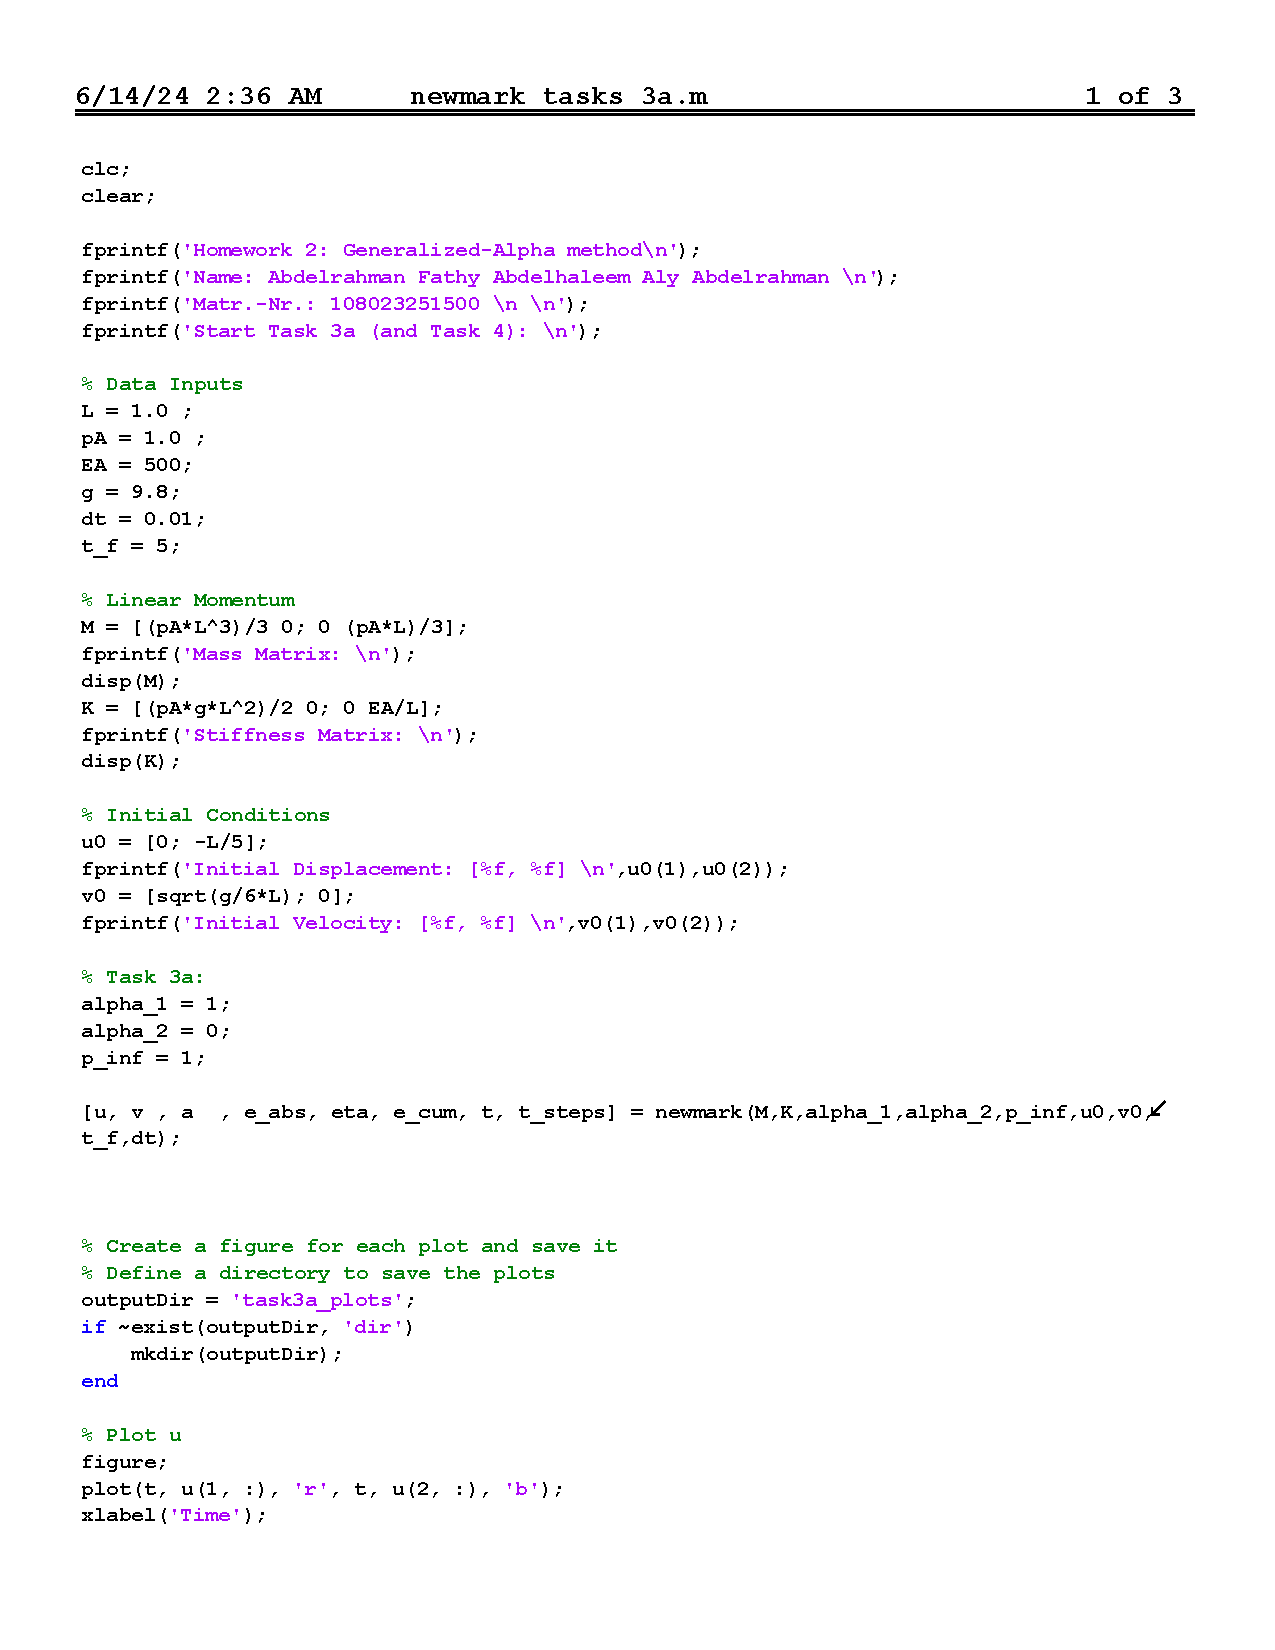
\includepdf[pages=-]{../newmark_tasks_3a.pdf}
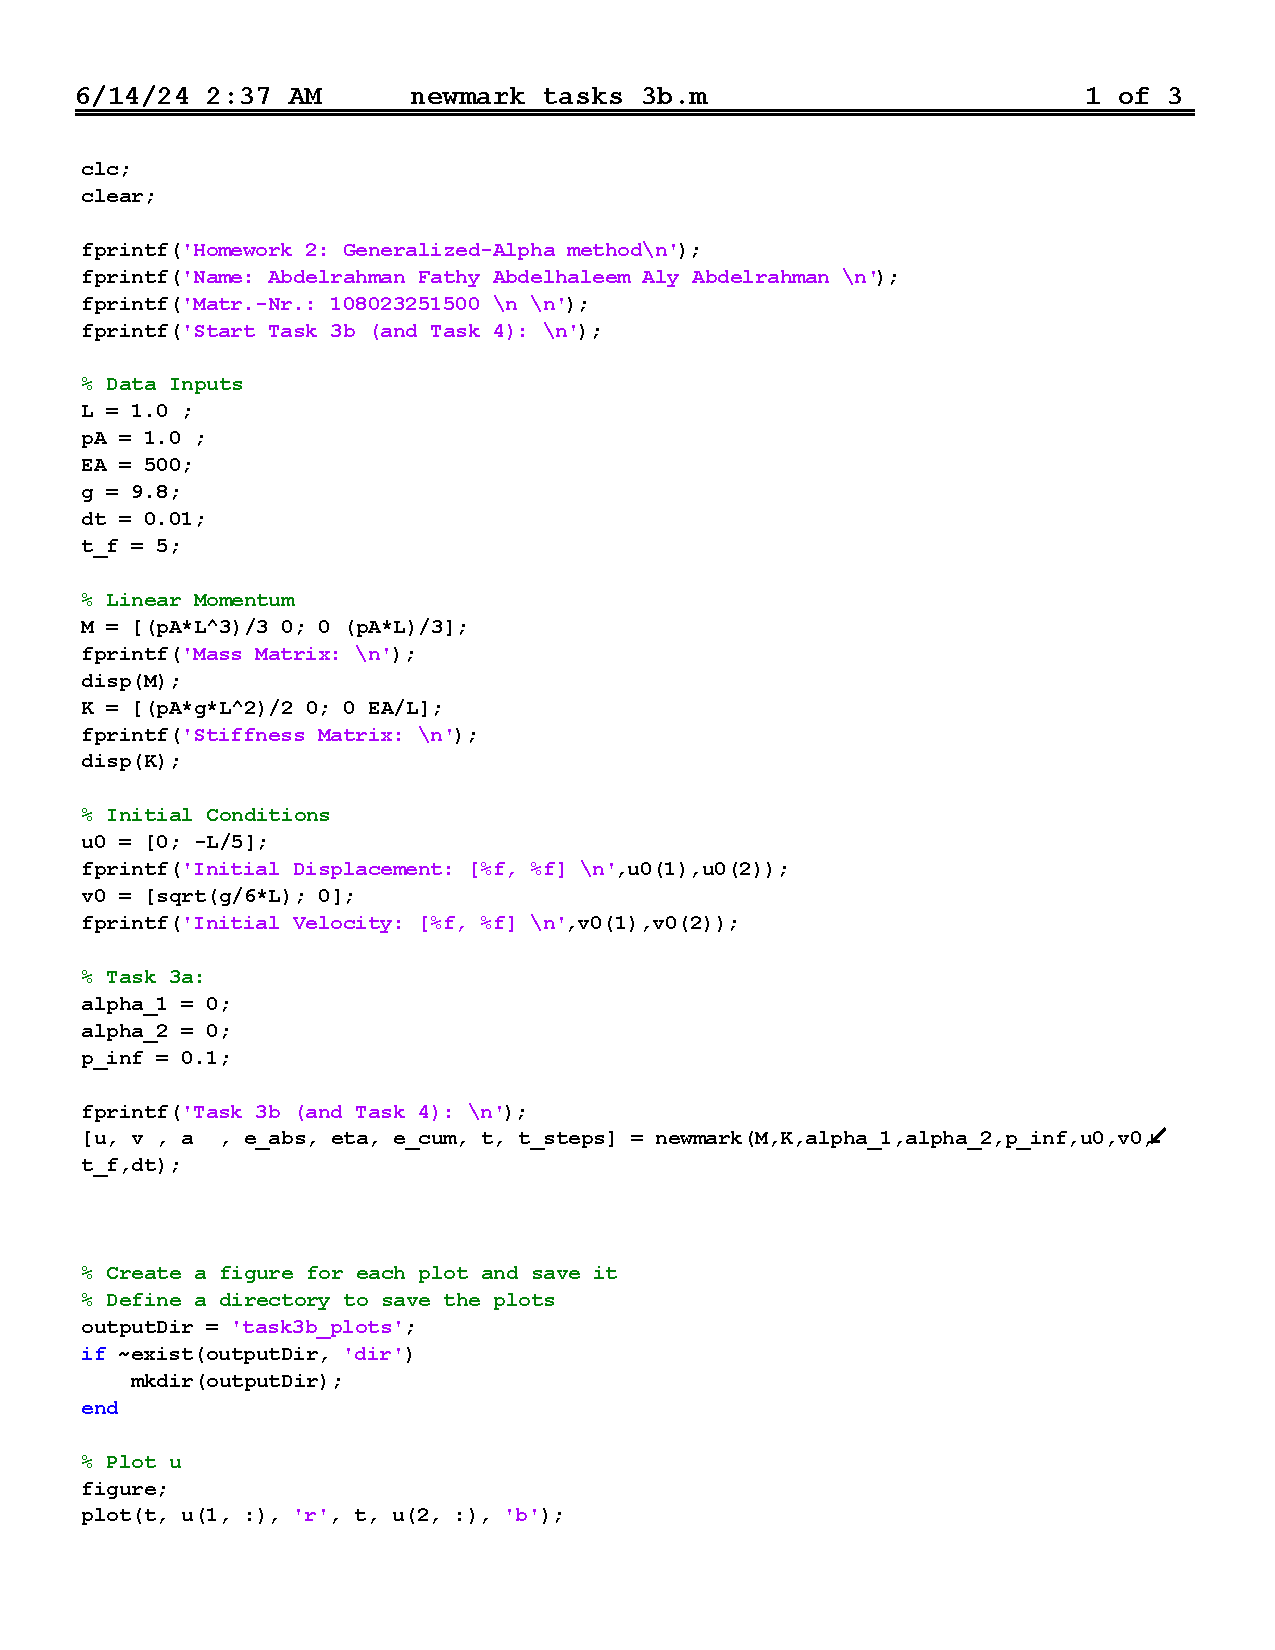
\includepdf[pages=-]{../newmark_tasks_3b.pdf}
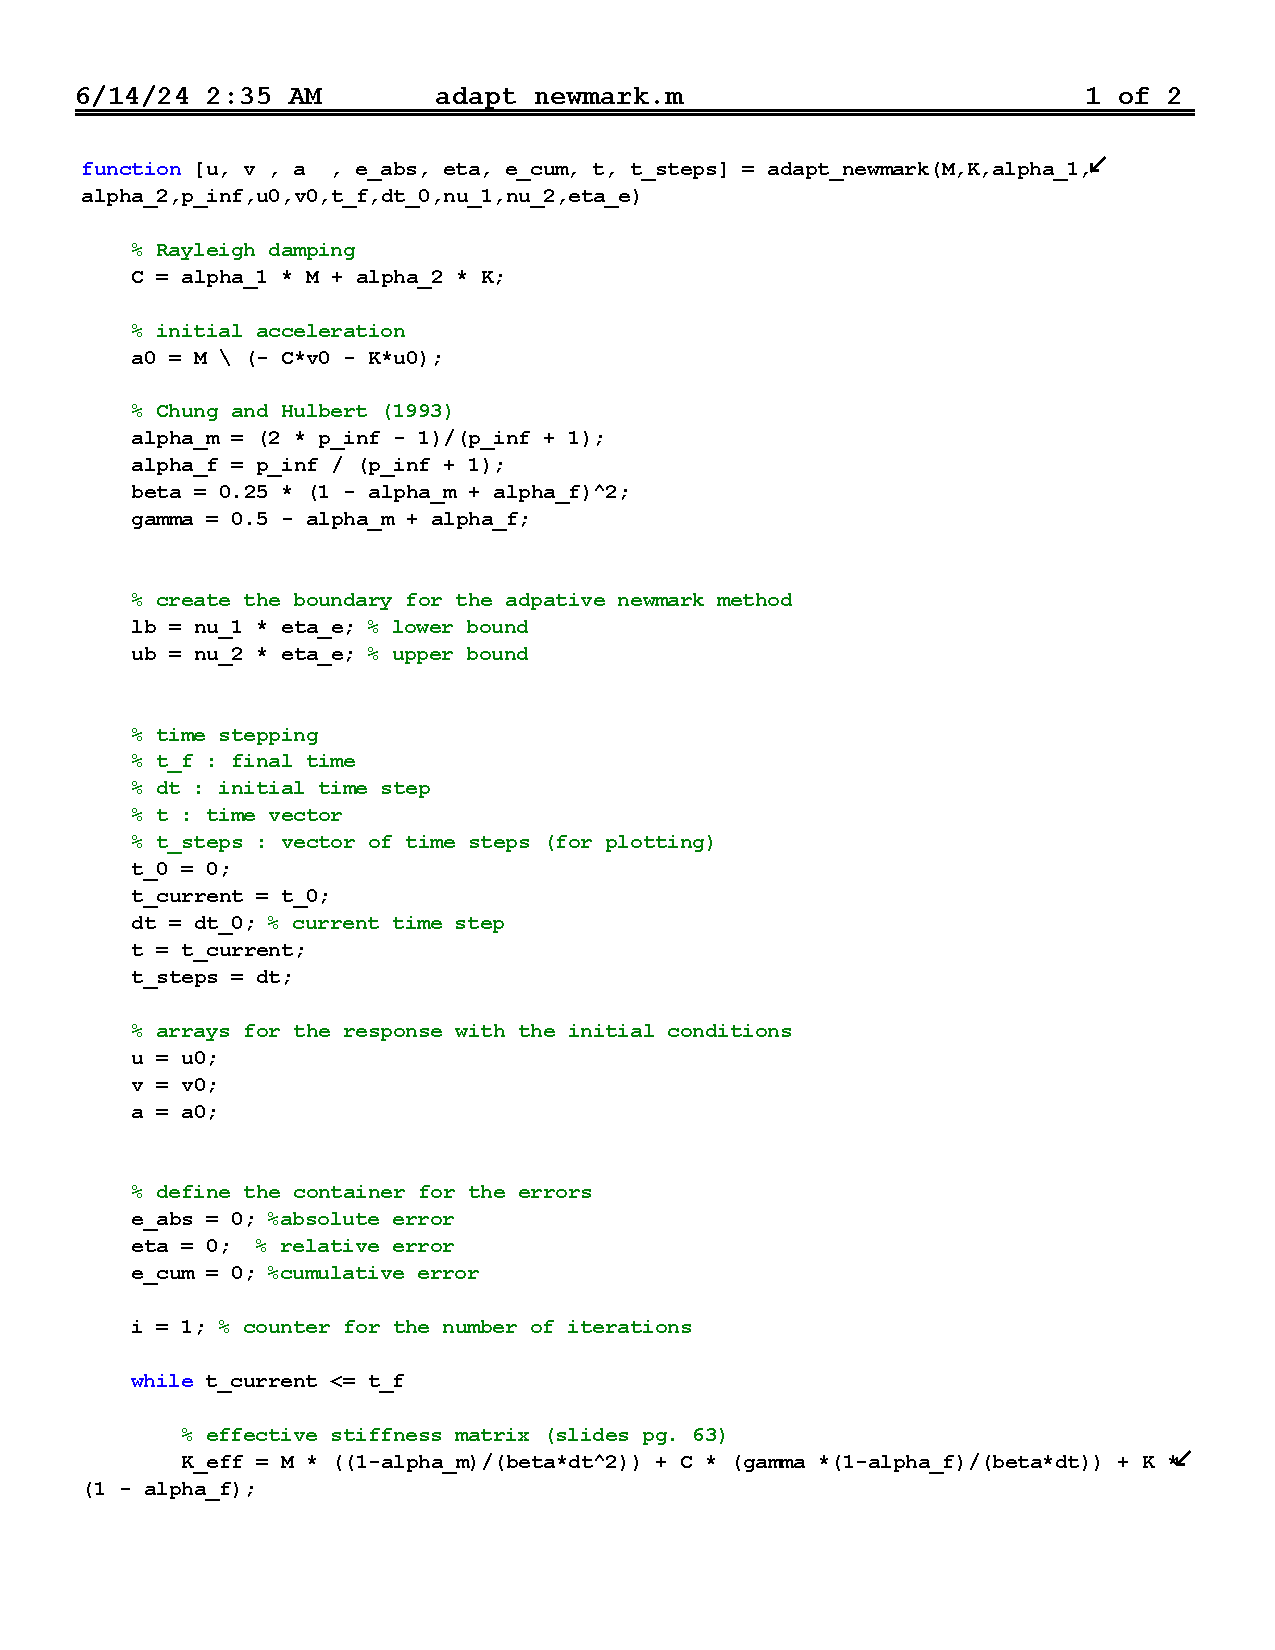
\includepdf[pages=-]{../adapt_newmark.pdf}
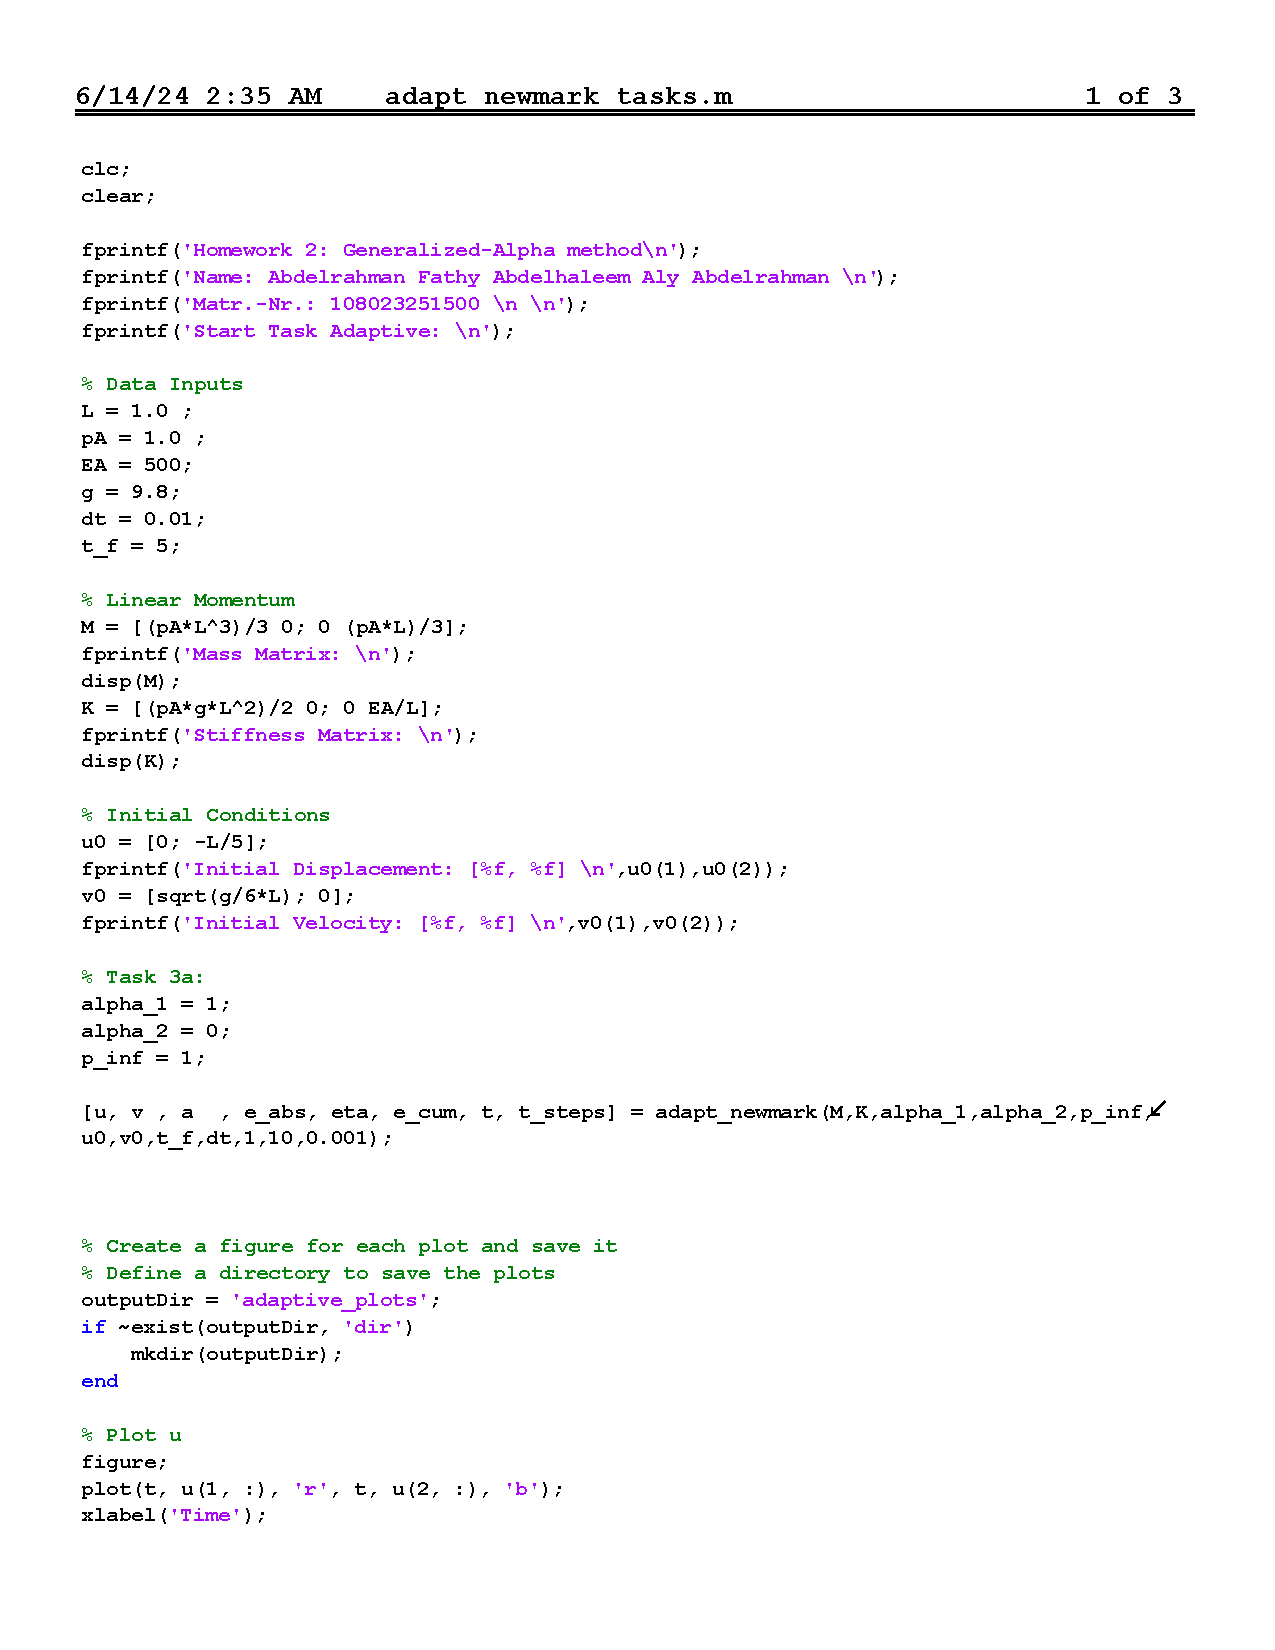
\includepdf[pages=-]{../adapt_newmark_tasks.pdf}

\newgeometry{left=0.001in, right=0.001in, top=0.5in, bottom=1in}
\begin{figure}[h]
  \centering
  \begin{subfigure}[b]{0.5\textwidth}
      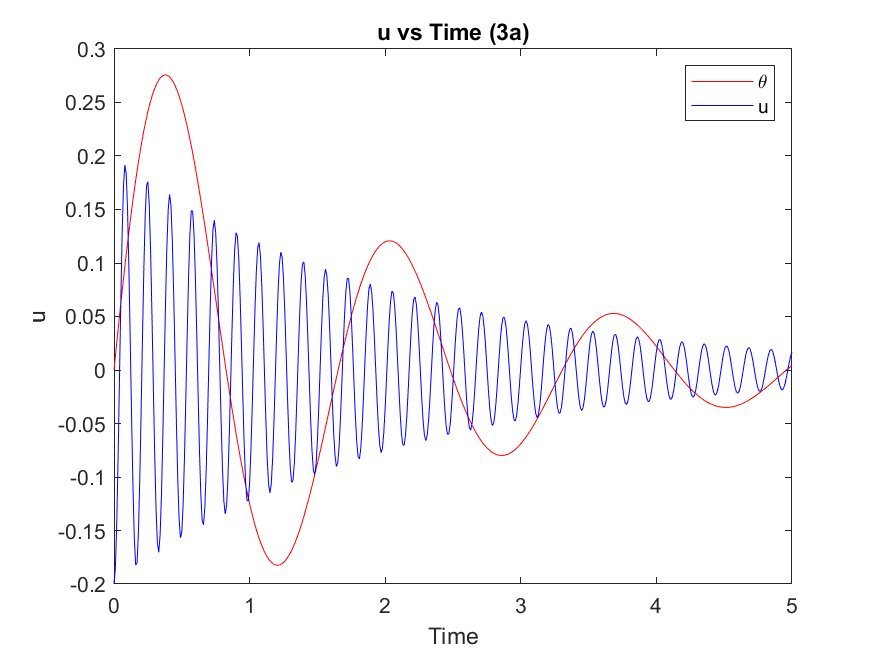
\includegraphics[width=\textwidth]{../../Matlab/task3a_plots/u_vs_time.png}
      \caption{displacement through time}
      \label{fig:image1}
  \end{subfigure}
  \hspace{-1.0em}% Adjust horizontal space between figures 
  \begin{subfigure}[b]{0.5\textwidth}
      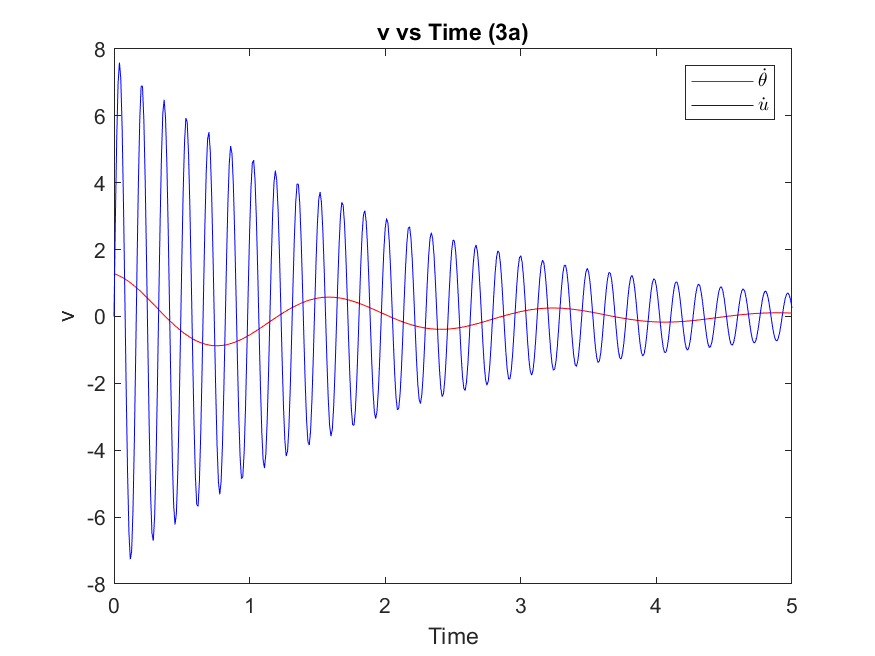
\includegraphics[width=\textwidth]{../../Matlab/task3a_plots/v_vs_time.png}
      \caption{velocity through time}
      \label{fig:image2}
  \end{subfigure}

  \vspace{0.5cm}

  \begin{subfigure}[b]{0.5\textwidth}
      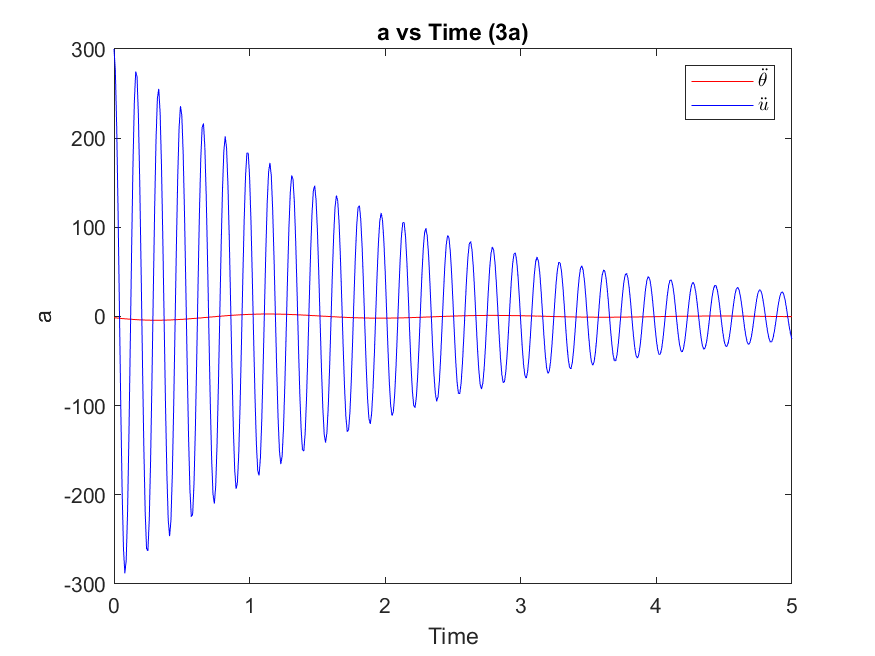
\includegraphics[width=\textwidth]{../../Matlab/task3a_plots/a_vs_time.png}
      \caption{acceleration through time}
      \label{fig:image3}
  \end{subfigure}
  \hfill
  
  \caption{Rsponse of the system for Task 3a}
  \label{fig:response_task3a}
\end{figure}

\newgeometry{left=0.001in, right=0.001in, top=0.5in, bottom=1in}

\begin{figure}[h]
  \centering
  \begin{subfigure}[b]{0.5\textwidth}
      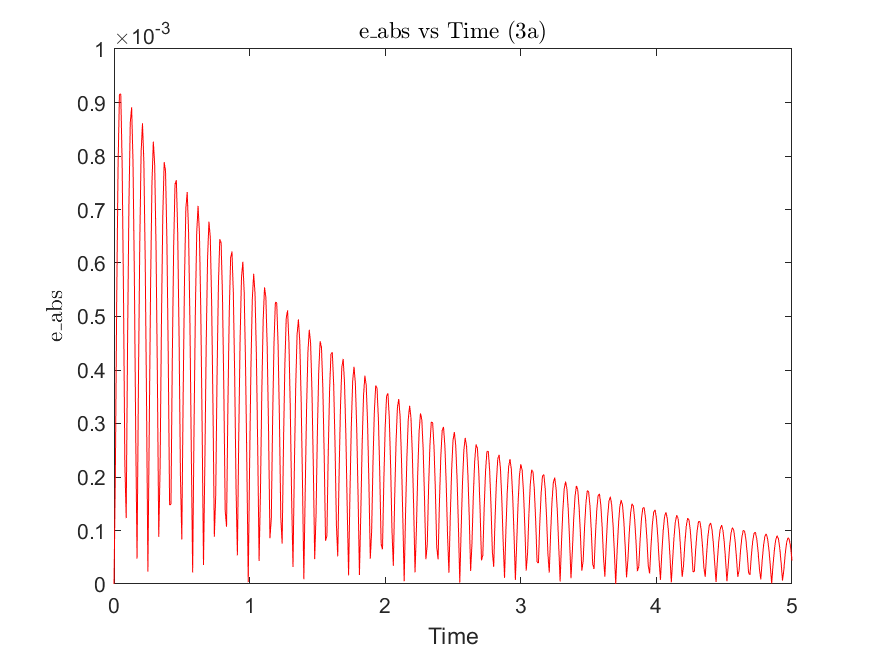
\includegraphics[width=\textwidth]{../../Matlab/task3a_plots/e_abs_vs_time.png}
      \caption{absolute error through time}
      \label{fig:image4}
  \end{subfigure}
  \hspace{-1.0em}% Adjust horizontal space between figures 
  \begin{subfigure}[b]{0.5\textwidth}
      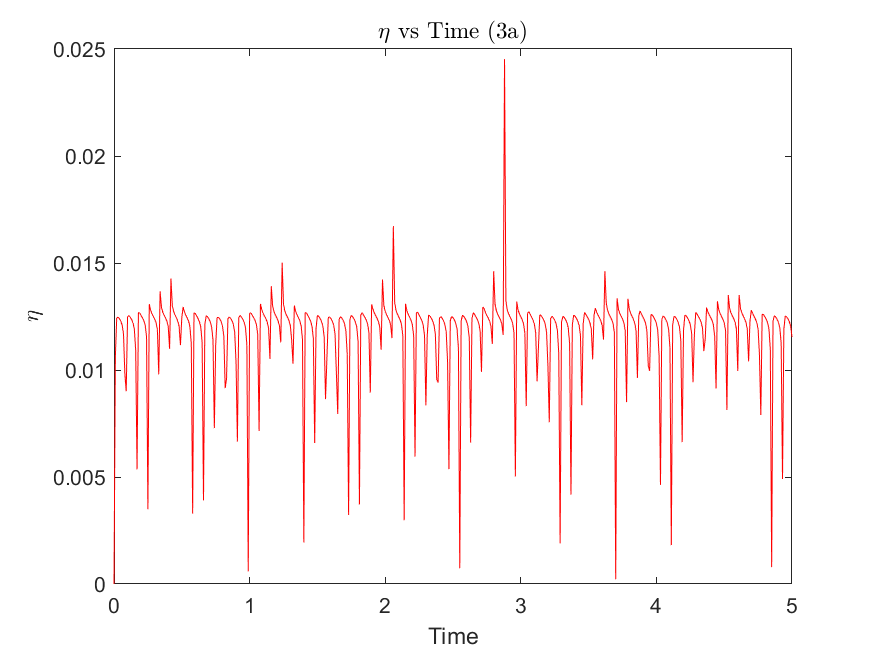
\includegraphics[width=\textwidth]{../../Matlab/task3a_plots/eta_vs_time.png}
      \caption{relative error through time}
      \label{fig:image5}
  \end{subfigure}

  \vspace{0.5cm}

  \begin{subfigure}[b]{0.5\textwidth}
      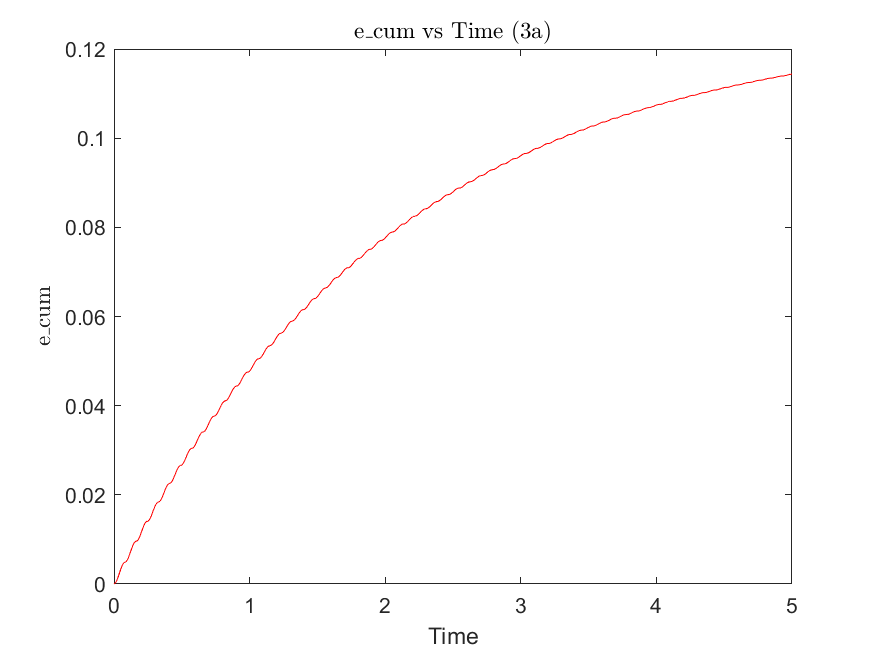
\includegraphics[width=\textwidth]{../../Matlab/task3a_plots/e_cum_vs_time.png}
      \caption{cumulative error through time}
      \label{fig:image6}
  \end{subfigure}
  \hfill
  
  \caption{errors in the system for Task 3a}
  \label{fig:error_task3a}
\end{figure}




%%%%%%%%%%%%%%%%%%%%%%%%%%%%%%%%%%%%%%%%%%%%%%%%%%%%%%%%%%%%
%% Task 3b
%%%%%%%%%%%%%%%%%%%%%%%%%%%%%%%%%%%%%%%%%%%%%%%%%%%%%%%%%%%%
\newgeometry{left=0.001in, right=0.001in, top=0.5in, bottom=1in}

\begin{figure}[h]
  \centering
  \begin{subfigure}[b]{0.5\textwidth}
      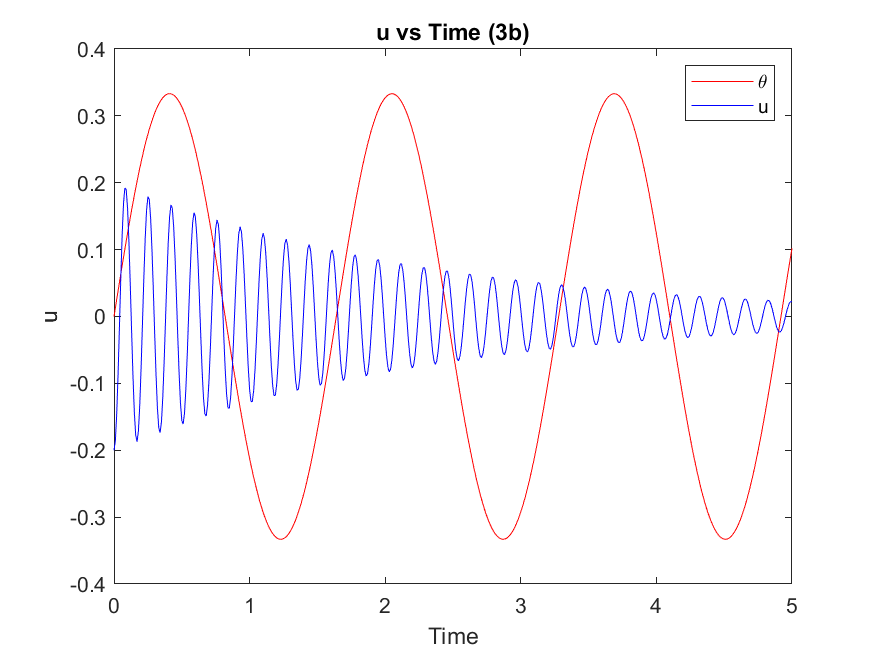
\includegraphics[width=\textwidth]{../../Matlab/task3b_plots/u_vs_time.png}
      \caption{displacement through time}
      \label{fig:image7}
  \end{subfigure}
  \hspace{-1.0em}% Adjust horizontal space between figures 
  \begin{subfigure}[b]{0.5\textwidth}
      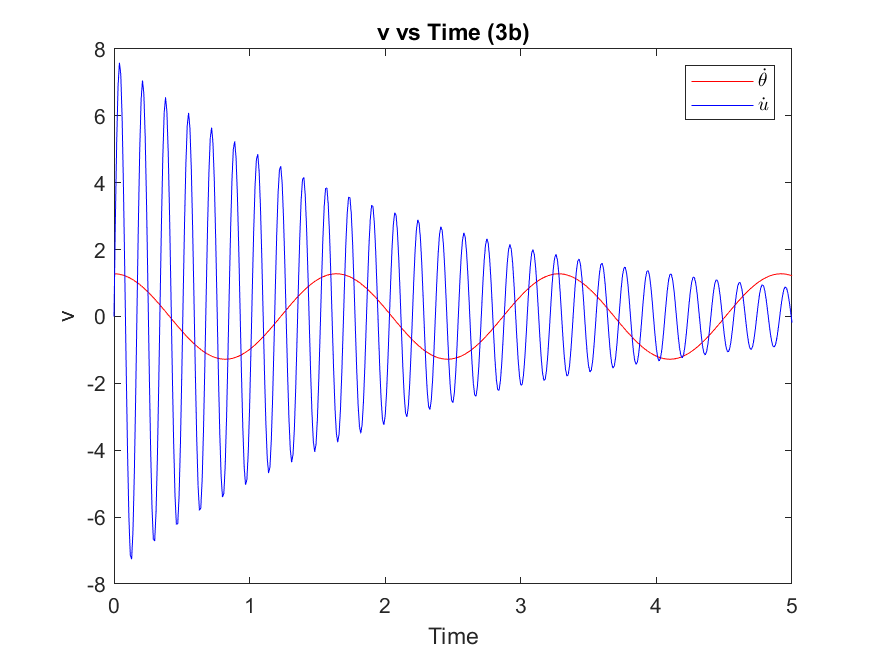
\includegraphics[width=\textwidth]{../../Matlab/task3b_plots/v_vs_time.png}
      \caption{velocity through time}
      \label{fig:image8}
  \end{subfigure}

  \vspace{0.5cm}

  \begin{subfigure}[b]{0.5\textwidth}
      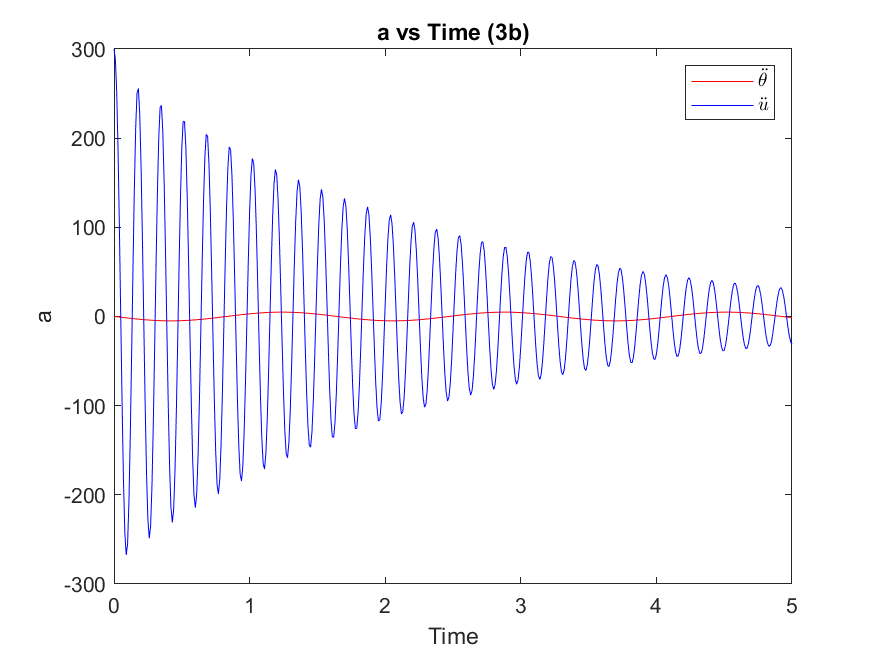
\includegraphics[width=\textwidth]{../../Matlab/task3b_plots/a_vs_time.png}
      \caption{acceleration through time}
      \label{fig:image9}
  \end{subfigure}
  \hfill
  
  \caption{Rsponse of the system for Task 3b}
  \label{fig:response_task3b}
\end{figure}

\newgeometry{left=0.001in, right=0.001in, top=0.5in, bottom=1in}

\begin{figure}[h]
  \centering
  \begin{subfigure}[b]{0.5\textwidth}
      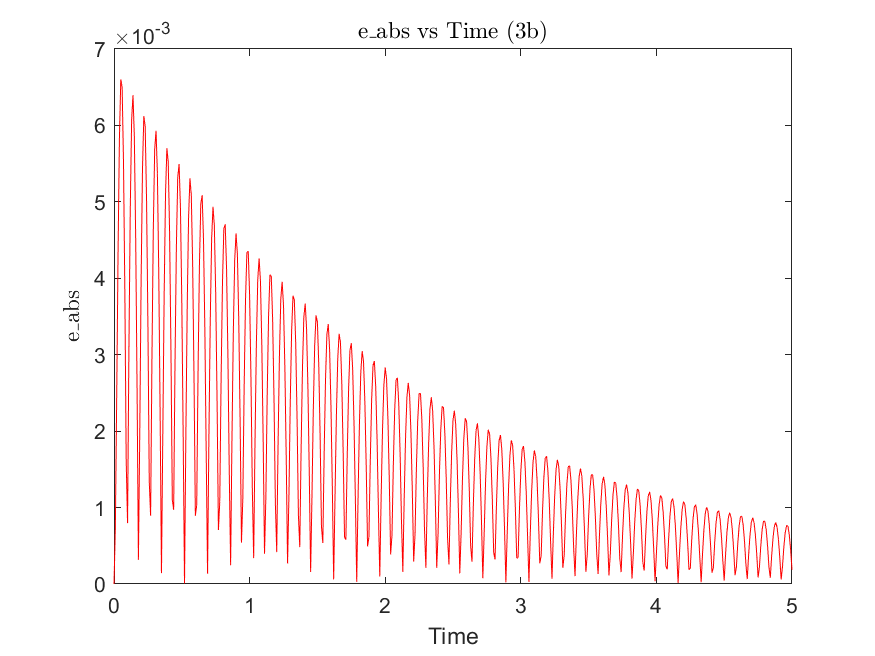
\includegraphics[width=\textwidth]{../../Matlab/task3b_plots/e_abs_vs_time.png}
      \caption{absolute error through time}
      \label{fig:image10}
  \end{subfigure}
  \hspace{-1.0em}% Adjust horizontal space between figures 
  \begin{subfigure}[b]{0.5\textwidth}
      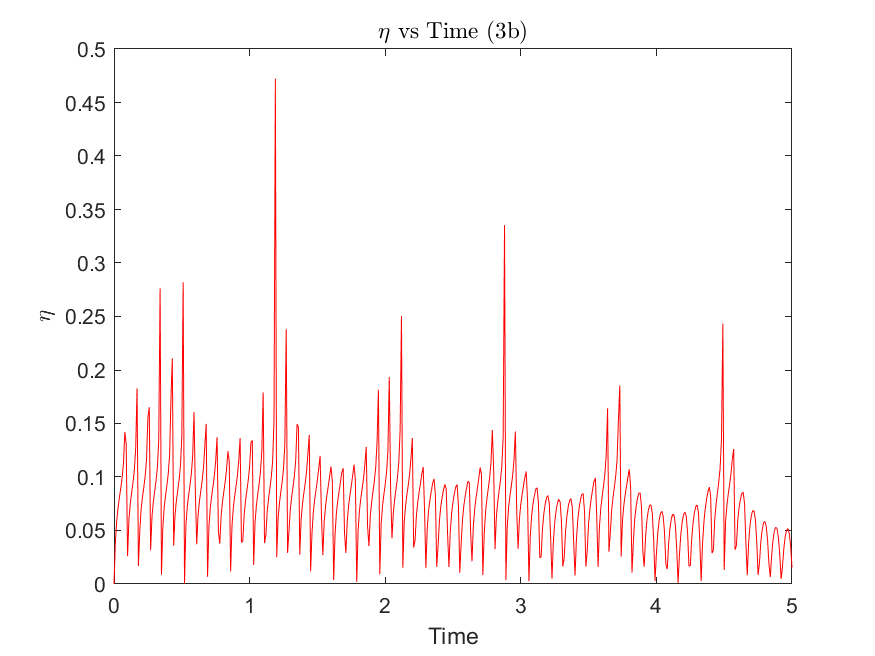
\includegraphics[width=\textwidth]{../../Matlab/task3b_plots/eta_vs_time.png}
      \caption{relative error through time}
      \label{fig:image11}
  \end{subfigure}

  \vspace{0.5cm}

  \begin{subfigure}[b]{0.5\textwidth}
      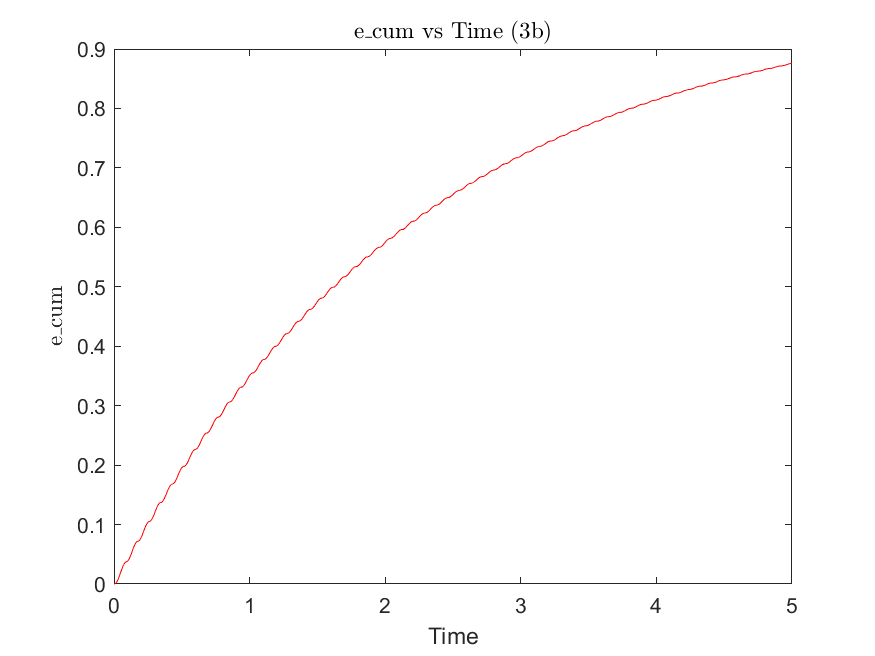
\includegraphics[width=\textwidth]{../../Matlab/task3b_plots/e_cum_vs_time.png}
      \caption{cumulative error through time}
      \label{fig:image12}
  \end{subfigure}
  \hfill
  
  \caption{errors in the system for Task 3b}
  \label{fig:error_task3b}
\end{figure}



%%%%%%%%%%%%%%%%%%%%%%%%%%%%%%%%%%%%%%%%%%%%%%%%%%%%%%%%%%%%
%% Adaptive Newmark
%%%%%%%%%%%%%%%%%%%%%%%%%%%%%%%%%%%%%%%%%%%%%%%%%%%%%%%%%%%%
\newgeometry{left=0.001in, right=0.001in, top=0.5in, bottom=1in}

\begin{figure}[h]
  \centering
  \begin{subfigure}[b]{0.5\textwidth}
      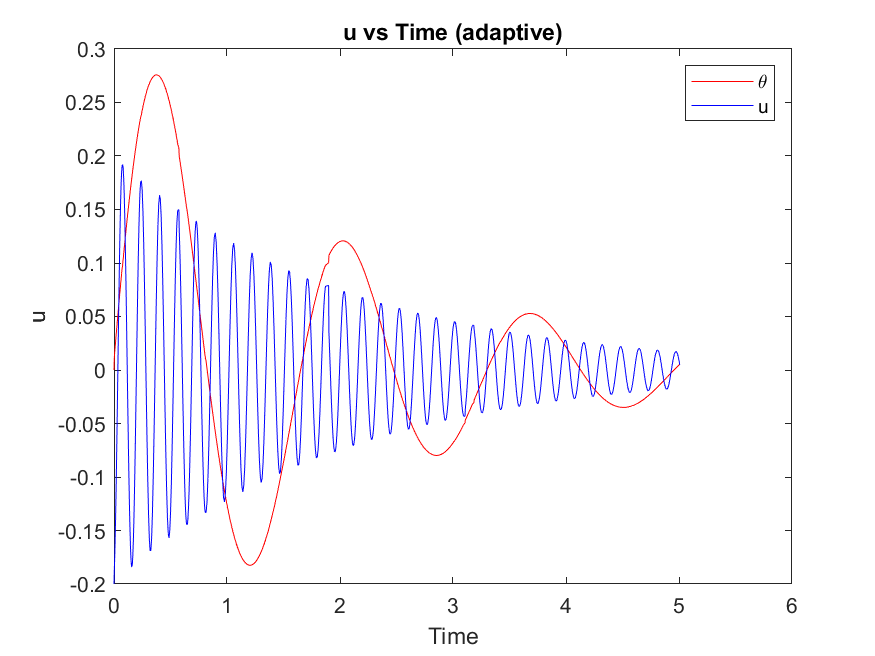
\includegraphics[width=\textwidth]{../../Matlab/adaptive_plots/u_vs_time.png}
      \caption{displacement through time}
      \label{fig:image13}
  \end{subfigure}
  \hspace{-1.0em}% Adjust horizontal space between figures 
  \begin{subfigure}[b]{0.5\textwidth}
      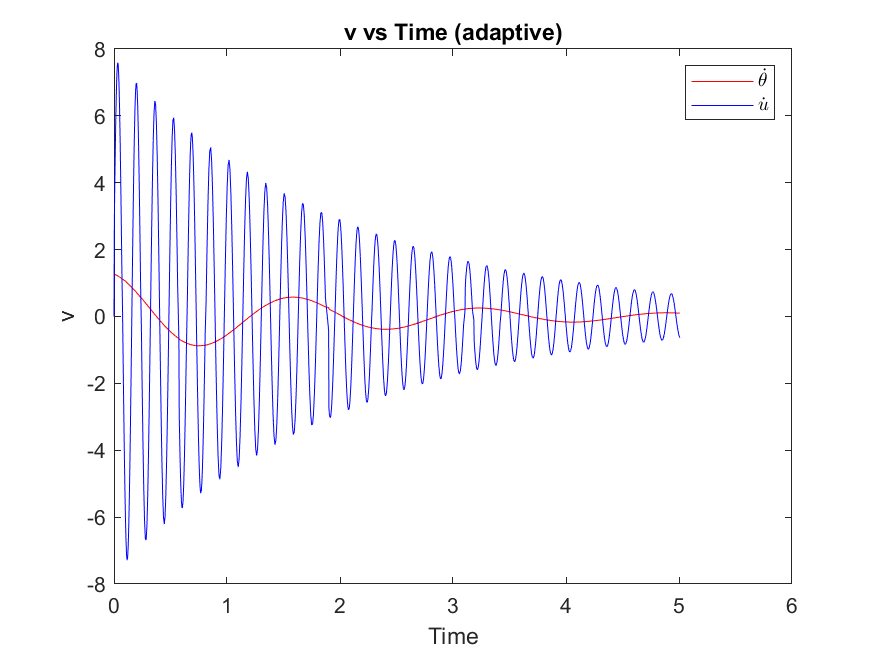
\includegraphics[width=\textwidth]{../../Matlab/adaptive_plots/v_vs_time.png}
      \caption{velocity through time}
      \label{fig:image14}
  \end{subfigure}

  \vspace{0.5cm}

  \begin{subfigure}[b]{0.5\textwidth}
      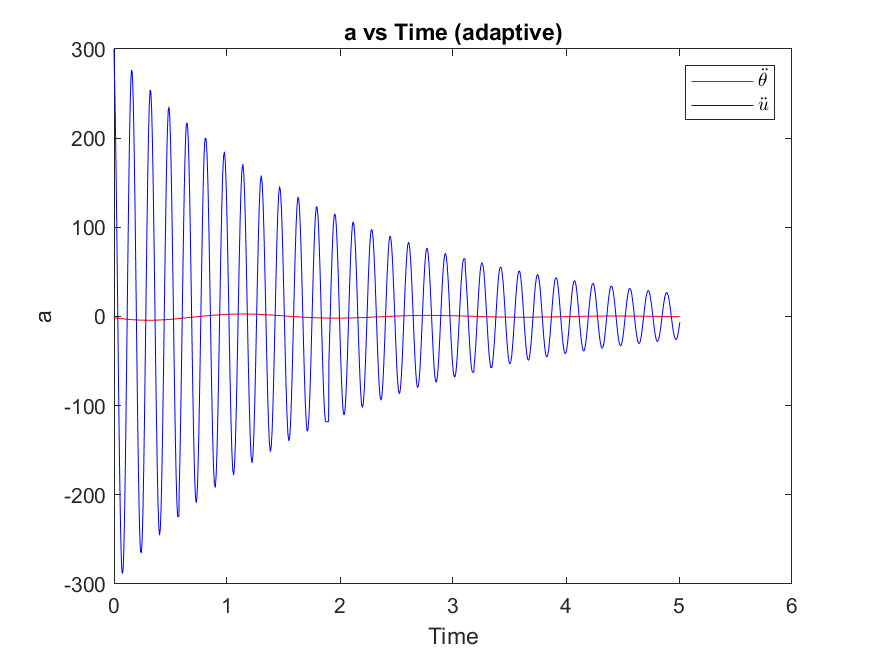
\includegraphics[width=\textwidth]{../../Matlab/adaptive_plots/a_vs_time.png}
      \caption{acceleration through time}
      \label{fig:image15}
  \end{subfigure}
  \hfill
  
  \caption{Rsponse of the system for Adaptive Newmark}
  \label{fig:response_adapt_newmark}
\end{figure}

\newgeometry{left=0.001in, right=0.001in, top=0.5in, bottom=1in}

\begin{figure}[h]
  \centering
  \begin{subfigure}[b]{0.5\textwidth}
      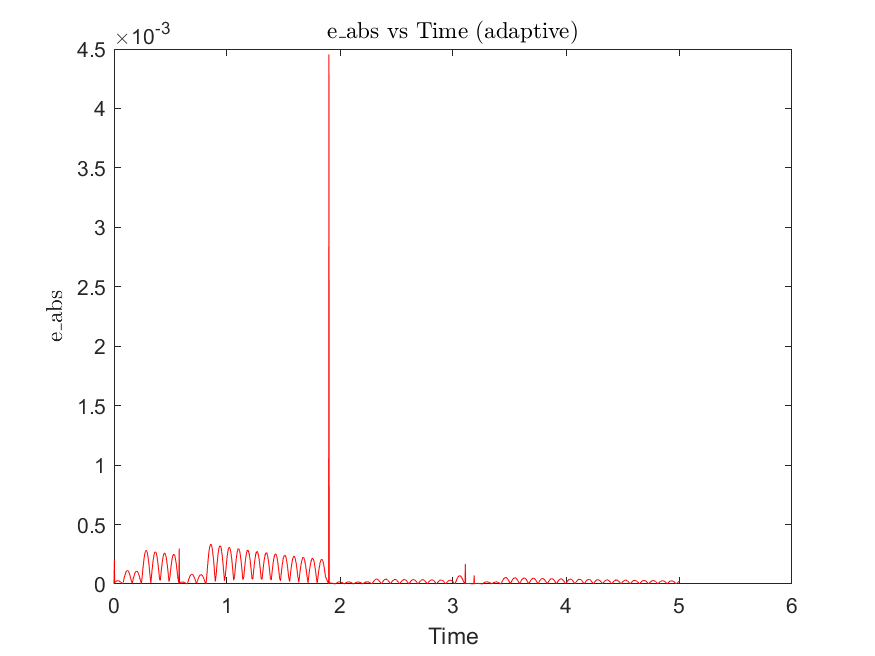
\includegraphics[width=\textwidth]{../../Matlab/adaptive_plots/e_abs_vs_time.png}
      \caption{absolute error through time}
      \label{fig:image16}
  \end{subfigure}
  \hspace{-1.0em}% Adjust horizontal space between figures 
  \begin{subfigure}[b]{0.5\textwidth}
      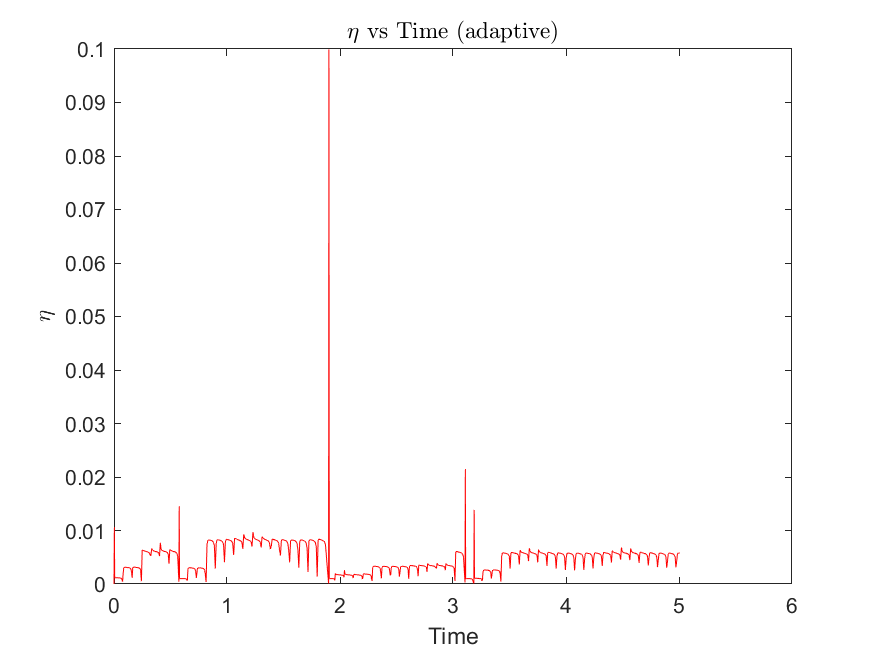
\includegraphics[width=\textwidth]{../../Matlab/adaptive_plots/eta_vs_time.png}
      \caption{relative error through time}
      \label{fig:image17}
  \end{subfigure}

  \vspace{0.5cm}

  \begin{subfigure}[b]{0.5\textwidth}
      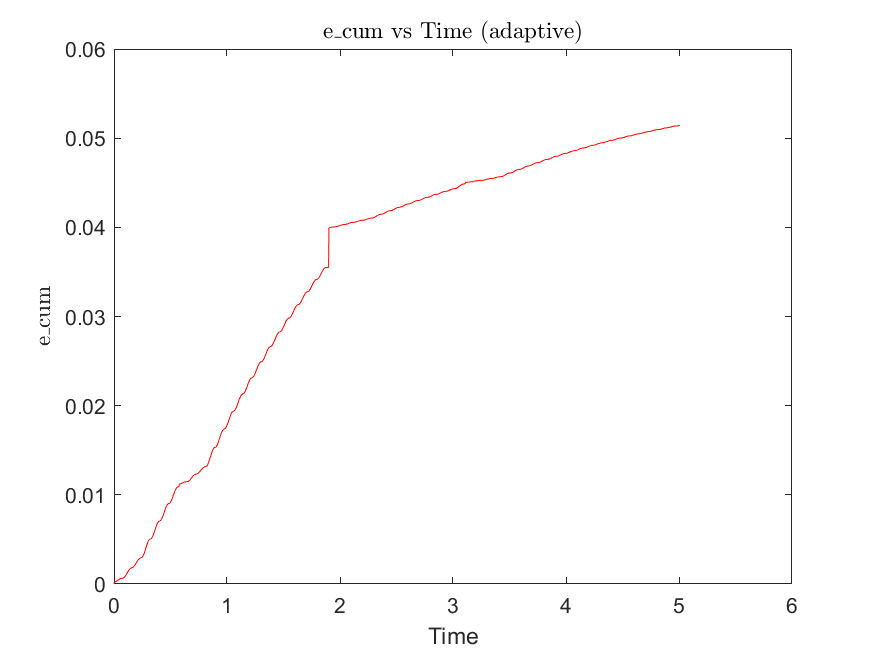
\includegraphics[width=\textwidth]{../../Matlab/adaptive_plots/e_cum_vs_time.png}
      \caption{cumulative error through time}
      \label{fig:image18}
  \end{subfigure}
  \hfill
  
  \caption{errors in the system for Adaptive Newmark}
  \label{fig:error_adapt_newmark}
\end{figure}





\end{document}